\documentclass[10pt]{article}
\usepackage{bookmark}
% Formato extenso: report

% Formato corto: article

% Esto es para que el LaTeX sepa que el texto está en español:
\usepackage[spanish]{babel}

\usepackage{amsmath, amsthm, amsfonts,amssymb}

% Bórrame si quieres:
\usepackage{multicol}

% Referencias
\usepackage{hyperref}

% Paquete para escribir código
\usepackage{listings}
\lstset{basicstyle=\footnotesize\ttfamily,breaklines=true}
\usepackage{alltt}

% Paquete para incluir imágenes
\usepackage{graphicx}

% Paquete para incluir varias imágenes en una
\usepackage{subfig}

% para poder fijar las imágenes ([H])
\usepackage{float}

% para agregar opciones al enumerate
\usepackage{enumerate}
\usepackage{tikz}
\usetikzlibrary{positioning}  % Carga las librerías necesarias

% Definir los estilos personalizados
\tikzstyle{block} = [draw, rectangle, minimum height=3em, minimum width=6em]
\tikzstyle{input} = [coordinate]
\tikzstyle{output} = [coordinate]
\tikzstyle{sum} = [draw, circle, node distance=1cm]

% Teoremas
\newtheorem{thm}{Teorema}[section]
\newtheorem{cor}[thm]{Corolario}
\newtheorem{lem}[thm]{Lema}
\newtheorem{prop}[thm]{Proposición}
\theoremstyle{definition}
\newtheorem{defn}[thm]{Definición}
\theoremstyle{remark}
\newtheorem{rem}[thm]{Observación}
\theoremstyle{definition}
\newtheorem{prob}{Problema}
\numberwithin{equation}{prob}

% Calculus symbols
\newcommand{\pd}[2]{\frac{\partial #1}{ \partial #2}}   % First partial derivative command
\newcommand{\td}[2]{\frac{\mathrm{d} #1}{ \mathrm{d} #2}}
\newcommand{\pdd}[2]{\frac{\partial^2 #1}{ \partial #2 ^2}}   % Second partial derivative command
\newcommand{\pddc}[3]{\frac{\partial^2 #1}{ \partial #2 \partial #3}}   % Second partial derivative command

% Continuum mechanics & FEM symbols
\def\sca   #1{\mbox{\rm{#1}}{}}
\def\mat   #1{\mbox{\boldmath $\mathsf #1$}}
\def\vec   #1{\mbox{\boldmath $#1$}{}}
\def\ten   #1{\mbox{\boldmath $#1$}{}}
\def\ltr   #1{\mbox{\sf{#1}}}
\def\bltr  #1{\mbox{\sffamily{\bfseries{{#1}}}}}

% math operators and symbols
\DeclareMathOperator{\dive}{div}
\DeclareMathOperator{\trace}{trace}
\DeclareMathOperator{\tr}{tr}
\DeclareMathOperator{\symm}{symm}
\DeclareMathOperator{\sk}{skew}
\DeclareMathOperator{\grad}{grad}
\DeclareMathOperator{\Grad}{Grad}
\DeclareMathOperator{\curl}{curl}
\DeclareMathOperator{\Curl}{Curl}
\def\R{\mbox{\(\mathbb{R}\)}}
\def\dx{\mbox{\(\,\mathrm{d}x\)}}


\usepackage{geometry}
\geometry{left=2.5cm, right=2.5cm, top=2cm, bottom=3cm}

\usepackage{makeidx}
\makeindex


\begin{document}

\begin{sloppypar}

\end{sloppypar}

\begin{titlepage}
	%%%%% NO MODIFICAR
	\begin{figure}
		\begin{minipage}{4cm}
			
\includegraphics[width=0.9\textwidth]{./figures/logo}
		\end{minipage}
		\begin{minipage}{11cm}
			\vspace{4mm}
			{\sc UNIVERSIDAD DE VALPARAÍSO}\\
			Escuela de Ingeniería Civil Biomédica\\
			{\bf CBM422 - Ingeniería de control automático}\\
			\vspace{0mm}
			\hrulefill
		\end{minipage}
	\end{figure}
	\phantom{""}\vspace{60mm}


	%%%%% MODIFICAR
	\begin{center}
		\Huge{\textbf{Tarea 1}}\vspace{95mm}\\
		\raggedleft \Large{Jorge Gonzalo Alejandro Alcaíno Brevis}\\
		\raggedleft \Large{Maximiliano Antonio Gaete Pizarro}\\
	\end{center}


\end{titlepage}

\index{entry}


\section{Problema 1: Encuentre las transformadas inversas de Laplace, de las siguientes funciones}

\begin{equation}
	\begin{aligned}
		\text{(a)} \quad F_1(s) & = \frac{6s + 3}{s^2}              \\
		\text{(b)} \quad F_2(s) & = \frac{5s + 2}{(s + 1)(s + 2)^2}
	\end{aligned}
\end{equation}


\subsection{Parte (a):}
\[
	F_1(s) = \frac{6s + 3}{s^2}
\]
Descomponiendo la función:
\[
	F_1(s) = 6 \cdot \frac{s}{s^2} + 3 \cdot \frac{1}{s^2}
\]
La transformada inversa de Laplace de cada término es:
\[
	\mathcal{L}^{-1}\left\{ \frac{s}{s^2} \right\} = 1, \quad \mathcal{L}^{-1}\left\{ \frac{1}{s^2} \right\} = t
\]
Por lo tanto, la transformada inversa de \( F_1(s) \) es:
\[
	\mathcal{L}^{-1}\left\{ F_1(s) \right\} = 6 + 3t
\]

\subsection{Parte (b):}
\[
	F_2(s) = \frac{5s + 2}{(s+1)(s+2)^2}
\]
Descomponiendo en fracciones parciales:
\[
	F_2(s) = \frac{-3}{s+1} + \frac{3}{s+2} + \frac{8}{(s+2)^2}
\]
Para esta fracción racional más compleja, podemos aplicar descomposición en fracciones parciales. La forma general sería:
\[
	\frac{5s + 2}{(s + 1)(s + 2)^2} = \frac{A}{s+1} + \frac{B}{s+2} + \frac{C}{(s+2)^2}
\]
Primero, multiplicamos ambos lados por \( (s + 1)(s + 2)^2 \) para eliminar los denominadores:
\[
	5s + 2 = A(s + 2)^2 + B(s + 1)(s + 2) + C(s + 1)
\]

Resolviendo en Python
\begin{lstlisting}[language=Python]
    from sympy import symbols, Eq, solve

    # Definimos la variable s y los coeficientes A, B, C
    s = symbols('s')
    A, B, C = symbols('A B C')
    
    # Expresion original
    lhs = 5*s + 2
    
    # Expansion en fracciones parciales
    rhs = A*(s+2)**2 + B*(s+1)*(s+2) + C*(s+1)
    
    # Expandimos el lado derecho
    expanded_rhs = rhs.expand()
    
    # Igualamos ambos lados para resolver el sistema de ecuaciones
    equations = Eq(lhs, expanded_rhs)
    
    # Resolvemos para A, B y C
    coefficients = solve(equations, [A, B, C])
    coefficients
\end{lstlisting}

Expandiendo ambos lados y resolviendo para \( A \), \( B \), y \( C \), encontramos los coeficientes que necesitamos. Esto nos da la forma correcta para aplicar la transformada inversa de Laplace a cada término:
\[
	\frac{5s + 2}{(s+1)(s+2)^2} = \frac{-3}{s+1} + \frac{3}{s+2} + \frac{8}{(s+2)^2}
\]
Aplicando la transformada inversa de Laplace a cada término:
\[
	\mathcal{L}^{-1}\left\{ \frac{1}{s+1} \right\} = e^{-t}, \quad \mathcal{L}^{-1}\left\{ \frac{1}{s+2} \right\} = e^{-2t}, \quad \mathcal{L}^{-1}\left\{ \frac{1}{(s+2)^2} \right\} = t e^{-2t}
\]
Por lo tanto, la transformada inversa de \( F_2(s) \) es:
\[
	\mathcal{L}^{-1}\left\{ F_2(s) \right\} = -3 e^{-t} + 3 e^{-2t} + 8 t e^{-2t}
\]

\newpage

\section{Problema 2: Obtenga la Función de Transferencia del sistema definido por las ecuaciones}

\begin{equation}
	\begin{aligned}
		\begin{bmatrix}
			\dot{x}_1 \\
			\dot{x}_2 \\
			\dot{x}_3
		\end{bmatrix}
		 & =
		\begin{bmatrix}
			0  & 1  & 0  \\
			0  & 0  & 1  \\
			-2 & -4 & -6
		\end{bmatrix}
		\begin{bmatrix}
			x_1 \\
			x_2 \\
			x_3
		\end{bmatrix}
		+
		\begin{bmatrix}
			0 & 0 \\
			0 & 1 \\
			1 & 0
		\end{bmatrix}
		\begin{bmatrix}
			u_1 \\
			u_2
		\end{bmatrix}
		\\
		\begin{bmatrix}
			y_1 \\
			y_2
		\end{bmatrix}
		 & =
		\begin{bmatrix}
			1 & 0 & 0 \\
			0 & 1 & 0
		\end{bmatrix}
		\begin{bmatrix}
			x_1 \\
			x_2 \\
			x_3
		\end{bmatrix}
	\end{aligned}
\end{equation}

\subsection{Obtención de la función de transferencia del sistema:}

Dado el sistema de ecuaciones en el espacio de estados:

\[
	\dot{\mathbf{x}}(t) = A\mathbf{x}(t) + B\mathbf{u}(t)
\]
\[
	\mathbf{y}(t) = C\mathbf{x}(t) + D\mathbf{u}(t)
\]

donde las matrices \( A \), \( B \), \( C \) y \( D \) están definidas como:

\[
	A = \begin{bmatrix}
		0  & 1  & 0  \\
		0  & 0  & 1  \\
		-2 & -4 & -6
	\end{bmatrix}, \quad
	B = \begin{bmatrix}
		0 & 0 \\
		0 & 1 \\
		1 & 0
	\end{bmatrix}, \quad
	C = \begin{bmatrix}
		1 & 0 & 0 \\
		0 & 1 & 0
	\end{bmatrix}, \quad
	D = \begin{bmatrix}
		0 & 0 \\
		0 & 0
	\end{bmatrix}
\]

La función de transferencia \( \mathbf{G}(s) \) en el dominio de Laplace se calcula utilizando la fórmula:

\[
	\mathbf{G}(s) = C(sI - A)^{-1}B + D
\]

Paso 1: Calcular \( (sI - A) \)

La matriz identidad \( I \) es:

\[
	I = \begin{bmatrix}
		1 & 0 & 0 \\
		0 & 1 & 0 \\
		0 & 0 & 1
	\end{bmatrix}
\]

Por lo tanto, \( (sI - A) \) es:

\[
	sI - A = \begin{bmatrix}
		s & -1 & 0     \\
		0 & s  & -1    \\
		2 & 4  & s + 6
	\end{bmatrix}
\]

Paso 2: Inversa de \( (sI - A) \)

Ahora, calculamos la inversa de \( (sI - A) \):

Resolviendo en python
\begin{lstlisting}[language=Python]
    from sympy import Matrix, eye, symbols, simplify

    # Definir las matrices y la variable s
    s = symbols('s')
    A = Matrix([[0, 1, 0], [0, 0, 1], [-2, -4, -6]])
    B = Matrix([[0, 0], [0, 1], [1, 0]])
    C = Matrix([[1, 0, 0], [0, 1, 0]])
    D = Matrix([[0, 0], [0, 0]])
    I = eye(3)  # Matriz identidad de 3x3
    
    # Calcular (sI - A) y su inversa
    sI_A_inv = (s * I - A).inv()
\end{lstlisting}

\[
	(sI - A)^{-1} = \frac{1}{s^3 + 6s^2 + 4s + 2} \begin{bmatrix}
		s^2 + 6s + 4 & s + 6        & 1        \\
		2s + 4       & s^2 + 6s + 2 & s + 6    \\
		2            & 2s + 4       & s^2 + 6s
	\end{bmatrix}
\]

Paso 3: Multiplicación con \( B \)

Multiplicamos \( (sI - A)^{-1} \) por \( B \):

\[
	(sI - A)^{-1}B = \frac{1}{s^3 + 6s^2 + 4s + 2} \begin{bmatrix}
		1 & s + 6    \\
		s & s(s + 6)
	\end{bmatrix}
\]

Paso 4: Multiplicación con \( C \) y adición de \( D \)

Finalmente, multiplicamos por \( C \) y sumamos \( D \), obteniendo la función de transferencia:

Resolviendo en Python
\begin{lstlisting}[language=Python]
    # Calcular la funcion de transferencia G(s) = C(sI - A)^(-1)B + D
    G_s = simplify(C * sI_A_inv * B + D)
    G_s
\end{lstlisting}
\[
	\mathbf{G}(s) = \begin{bmatrix}
		\frac{1}{s^3 + 6s^2 + 4s + 2} & \frac{s + 6}{s^3 + 6s^2 + 4s + 2}    \\
		\frac{s}{s^3 + 6s^2 + 4s + 2} & \frac{s(s + 6)}{s^3 + 6s^2 + 4s + 2}
	\end{bmatrix}
\]

Esta es la función de transferencia del sistema, que describe la relación entre las entradas \( u_1 \) y \( u_2 \), y las salidas \( y_1 \) y \( y_2 \).

\newpage

\section{Problema 3: Mediante la simplificación del diagrama de bloques de la Figura 1, obtenga las siguientes funciones de transferencia}

\[
	\frac{Y(s)}{R(s)} \bigg|_{N=0}
	\quad \quad
	\frac{Y(s)}{N(s)} \bigg|_{R=0}
\]

\begin{figure}[h]
	\centering
	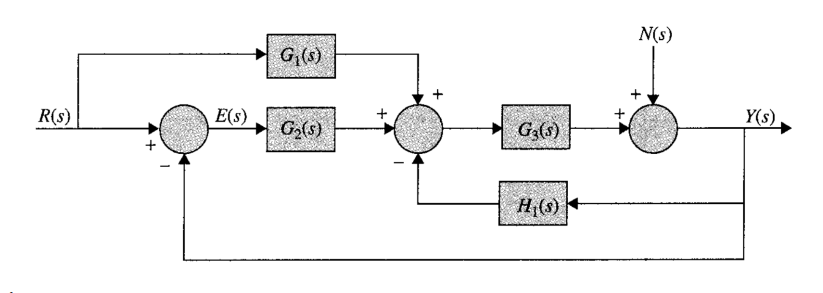
\includegraphics[width=0.9\textwidth]{./figures/Figura 1 ejercicio 3.png}
	\caption{Diagrama de bloques del sistema}
\end{figure}

\section{Problema 4: Obtenga la Función de Transferencia \texorpdfstring{$E_o(s)/E_i(s)$}{Eo(s)/Ei(s)} del circuito eléctrico RLC que se muestra en la Figura 2}

\begin{figure}[h]
	\centering
	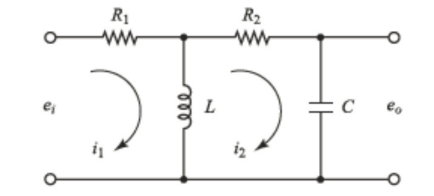
\includegraphics[width=0.6\textwidth]{./figures/Figura 2 ejercicio 4.png}
	\caption{Circuito eléctrico RLC}
\end{figure}

\subsection*{Primera malla}

\[
	R_1 i_1(t) + L \frac{d}{dt} \left( i_1(t) - i_2(t) \right) = e_i(t)
\]

Aplicamos la transformada de Laplace:

\[
	R_1 I_1(s) + Ls \left( I_1(s) - I_2(s) \right) = E_i(s)
\]

Despejamos $I_1(s)$:

\[
	I_1(s) = \frac{E_i(s) + Ls I_2(s)}{R_1 + Ls}
\]

\subsection*{Segunda malla}

\[
	L \frac{d}{dt} \left( i_2(t) - i_1(t) \right) + R_2 i_2(t) + \frac{1}{C} \int i_2(t) \, dt = 0
\]

Aplicamos la transformada de Laplace:

\[
	Ls \left( I_2(s) - I_1(s) \right) + R_2 I_2(s) + \frac{1}{Cs} I_2(s) = 0
\]

Despejamos $I_2(s)$:

\[
	I_2(s) = \frac{LCs^2}{(LCs^2 + R_2 Cs + 1)} I_1(s)
\]

\subsection*{Tercera malla}

\[
	\frac{1}{C} \int i_2(t) \, dt = e_0(t)
\]

En el dominio de Laplace:

\[
	\frac{1}{Cs} I_2(s) = E_0(s)
\]

% Primer bloque
\begin{tikzpicture}[auto, node distance=2cm, >=latex]
	\node [input, name=input] {};
	\node [sum, right of=input] (sum) {};
	\node [block, right of=sum] (controller) {$\displaystyle \frac{1}{R_1 + Ls}$};
	\node [block, right of=controller, node distance=3cm] (system) {$\displaystyle \frac{Ls^2}{LCs^2 + R_2Cs + 1}$};
	\node [output, right of=system] (output) {};
	\node [block, below of=system, node distance=1.5cm] (measurements) {$\displaystyle Ls$};

	\draw [->] (input) -- node {$E_i(s)$} (sum);
	\draw [->] (sum) -- (controller);
	\draw [->] (controller) -- (system);
	\draw [->] (system) -- (output);
	\draw [->] (output) |- (measurements);
	\draw [->] (measurements) -| node[pos=0.99] {$+$} (sum);

	\node [block, right of=output, node distance=3cm] (newblock) {$\displaystyle \frac{1}{Cs}$};
	\node [output, right of=newblock, node distance=2cm] (outputEo) {};

	\draw [->] (output) -- (newblock);
	\draw [->] (newblock) -- node {$E_o(s)$} (outputEo);
\end{tikzpicture}

\vspace{1cm}

% Segundo bloque
\begin{tikzpicture}[auto, node distance=5cm, >=latex']
    \node [input, name=input] {};
    \node [block, right of=input, minimum width=5cm] (formula) {
        \centering
        $\displaystyle \frac{LCs^2}{(LCs^2 + R_2Cs + 1)(R_1 + Ls) - L^2Cs^3}$
    };
    \node [block, right of=formula, minimum width=3cm] (inverse) {$\displaystyle \frac{1}{Cs}$};
    \node [output, right of=inverse] (output) {};

    \draw [->] (input) -- node {$E_i(s)$} (formula);
    \draw [->] (formula) -- (inverse);
    \draw [->] (inverse) -- node {$E_0(s)$} (output);
\end{tikzpicture}

\vspace{1cm}

% Tercer bloque
\begin{tikzpicture}[auto, node distance=4cm, >=latex']
    \node [input, name=input] {};
    \node [block, right of=input, minimum width=5cm] (formula) {
        \centering
        $\displaystyle \frac{Ls}{(R_1LC + R_2LC)s^2 + (R_1R_2C + L)s + R_1}$
    };

    \draw [->] (input) -- node {$E_i(s)$} (formula);
    \draw [->] (formula.east) -- ++(1,0) node[right] {$E_0(s)$};
\end{tikzpicture}


\section{Problema 5: Considere el sistema de la Figura 3(a). El factor de amortiguamiento relativo \texorpdfstring{$\zeta$}{}
  del sistema es igual a 0,158, y la frecuencia natural no amortiguada \texorpdfstring{$\omega_n$}{omega\_n} es de 3,16 rad/seg.
  Para mejorar la estabilidad se emplea una segunda retroalimentación, como se muestra en la
  Figura 3(b).
  Determine el valor de \texorpdfstring{$K_h$}{Kh}, para que el factor de amortiguamiento relativo del sistema sea ahora
  0,5. Obtenga la curva de respuesta al escalón unitario (analítica y computacionalmente), tanto
  del sistema original como del sistema con la nueva retroalimentación. Y analice.}

\begin{figure}[h]
	\centering
	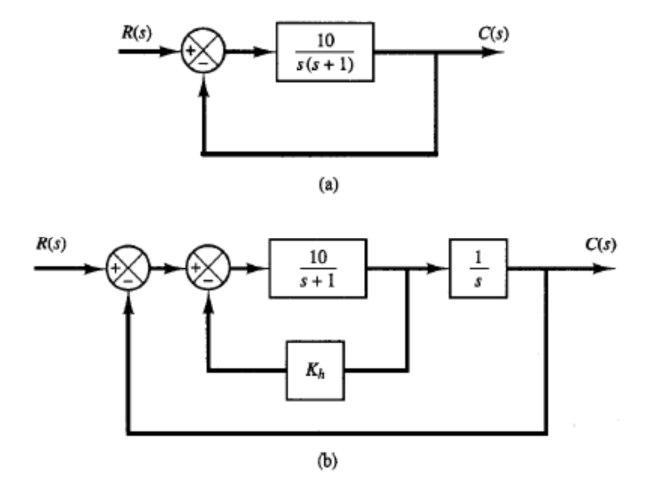
\includegraphics[width=0.8\textwidth]{./figures/Figura 3 ejercicio 5.png}
	\caption{Sistema de la Figura 3(a) y 3(b)}
\end{figure}


\subsection{El sistema dado en la Figura 3(a) tiene la siguiente función de transferencia:}

\[
	G(s) = \frac{10}{s(s + 1)}
\]

Con una retroalimentación unitaria, la función de transferencia de lazo cerrado es:

\[
	T(s) = \frac{G(s)}{1 + G(s)} = \frac{\frac{10}{s(s+1)}}{1 + \frac{10}{s(s+1)}} = \frac{10}{s^2 + s + 10}
\]

De acuerdo a los datos proporcionados:

\begin{itemize}
	\item El factor de amortiguamiento relativo (\(\zeta\)) es \(0.158\).
	\item La frecuencia natural no amortiguada (\(\omega_n\)) es \(3.16 \, \text{rad/seg}\).
\end{itemize}

Estos parámetros corresponden a una ecuación característica de segundo orden de la forma:

\[
	s^2 + 2\zeta \omega_n s + \omega_n^2 = 0
\]

Sustituyendo los valores:

\[
	s^2 + 2(0.158)(3.16)s + (3.16)^2 = s^2 + 0.998s + 9.9856
\]

Lo cual se aproxima bastante a la ecuación característica del sistema de lazo cerrado original: \(s^2 + s + 10\).


Implementación computacional en Python
\begin{lstlisting}[language=Python]
	import control as ctrl
	import matplotlib.pyplot as plt
	
	# Sistema original
	num_orig = [10]
	den_orig = [1, 1, 10]
	sys_orig = ctrl.TransferFunction(num_orig, den_orig)

	# Simulacion de la respuesta al escalon
	t, y_orig = ctrl.step_response(sys_orig)

	# Graficar resultados
	plt.plot(t, y_orig, color='b', label='Sistema Original')
	plt.title('Respuesta al escalon unitario')
	plt.xlabel('Tiempo (s)')
	plt.ylabel('Respuesta')
	plt.legend()
	plt.grid()
	plt.show()
\end{lstlisting}

\begin{figure}[h]
	\centering
	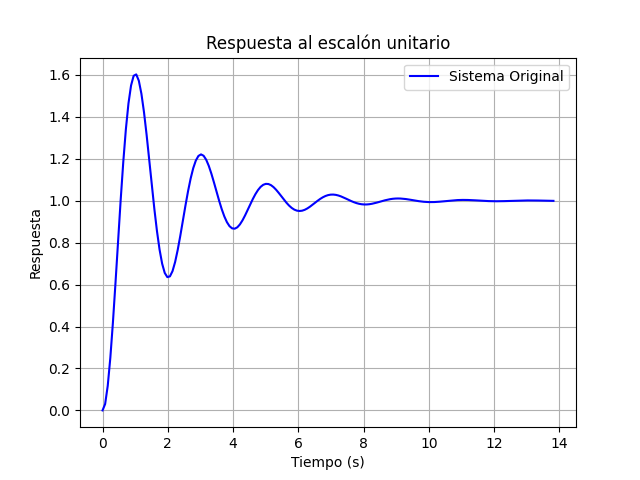
\includegraphics[width=0.7\textwidth]{./figures/Figura 4 ejercicio 5.png}
	\caption{Respuesta al escalón unitario del sistema original}
\end{figure}

\subsection{Sistema con nueva retroalimentación (Figura 3b)}

En la Figura 3(b), se añade una segunda retroalimentación con ganancia \(k\). Este valor se ajusta para lograr un coeficiente de amortiguamiento deseado de \( \zeta = 0.5 \). La nueva función de transferencia será:

\[
	T(s) = \frac{10}{s^2 + (10k + 1)s + 10}
\]

El polinomio característico de un sistema de segundo orden es:

\[
	s^2 + 2\zeta \omega_n s + \omega_n^2
\]

Al comparar ambos polinomios:

\[
	s^2 + (10k + 1)s + 10 = s^2 + 2\zeta \omega_n s + \omega_n^2
\]

De esta comparación, obtenemos dos ecuaciones:

\begin{itemize}
	\item Para el término de \( s \): \( 2\zeta \omega_n = 10k + 1 \)
	\item Para el término constante: \( \omega_n^2 = 10 \)
\end{itemize}

\subsubsection{Cálculo de \texorpdfstring{\( \omega_n \)}{omega\_n}}

A partir de \( \omega_n^2 = 10 \), tenemos que:

\[
	\omega_n = \sqrt{10}
\]

\subsubsection{Cálculo de \texorpdfstring{\( k \)}{k}}

Usando la ecuación para el coeficiente de amortiguamiento, \( 2\zeta \omega_n = 10k + 1 \), y sustituyendo \( \zeta = 0.5 \) y \( \omega_n = \sqrt{10} \):

\[
	2(0.5)\sqrt{10} = 10k + 1
\]

Despejando para \( k \):

\[
	k = \frac{2(0.5)\sqrt{10} - 1}{10}
\]

Finalmente, obtenemos el valor de \( k \):

\[
	k \approx 0.2162
\]

Implementación computacional en Python
\begin{lstlisting}[language=Python]
	import control as ctrl
	import matplotlib.pyplot as plt

	# Sistema con nueva retroalimentacion
	k = 0.2162
	num_new = [10]
	den_new = [1, (10*k+1), 10]
	sys_new = ctrl.TransferFunction(num_new, den_new)

	t2, y_new = ctrl.step_response(sys_new)

	# Graficar resultados
	plt.plot(t2, y_new, color='r', label='Sistema con nueva retroalimentacion')
	plt.title('Respuesta al escalon unitario')
	plt.xlabel('Tiempo (s)')
	plt.ylabel('Respuesta')
	plt.legend()
	plt.grid()
	plt.show()
\end{lstlisting}

\begin{figure}[h]
	\centering
	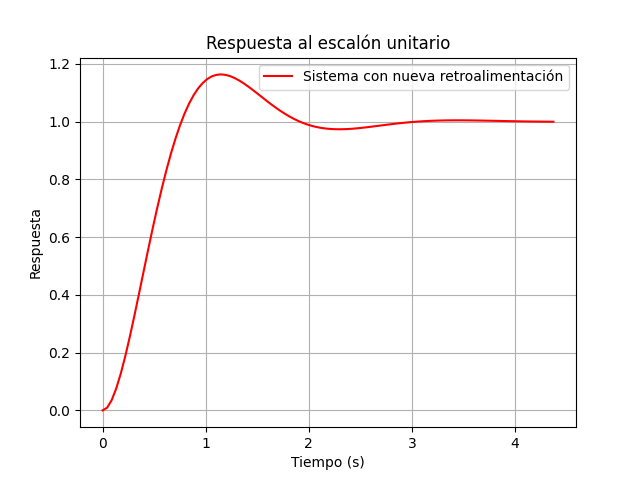
\includegraphics[width=0.7\textwidth]{./figures/Figura 5 ejercicio 5.png}
	\caption{Respuesta al escalón unitario del sistema con nueva retroalimentación}
\end{figure}

\newpage

\subsection{Respuesta al escalón unitario}

\subsection*{Sistema original}

La función de transferencia del sistema original es:

\[
	T(s) = \frac{10}{s^2 + s + 10}
\]

Usando la transformada inversa de Laplace, la respuesta al escalón unitario de este sistema presenta un comportamiento típico de un sistema de segundo orden subamortiguado, con un factor de amortiguamiento \(\zeta \approx 0.158\), lo que implica una respuesta con oscilaciones y una mayor sobreoscilación.

\subsection*{Sistema con retroalimentación ajustada}

Para el sistema con retroalimentación y el valor ajustado de \( k \), la función de transferencia se convierte en:

\[
	T_{\text{nuevo}}(s) = \frac{10}{s^2 + (10k + 1)s + 10}
\]

Sustituyendo \( k = 0.2162 \), obtenemos:

\[
	T_{\text{nuevo}}(s) = \frac{10}{s^2 + (10(0.2162) + 1)s + 10} = \frac{10}{s^2 + 3.162s + 10}
\]

Este sistema tiene un factor de amortiguamiento de \( \zeta = 0.5 \), lo que implica una mayor estabilidad y una reducción significativa en las oscilaciones en la respuesta al escalón unitario.

\subsection*{Análisis}

El sistema con la ganancia \( k \approx 0.2162 \) tiene una respuesta al escalón más rápida y con menos sobreoscilación en comparación con el sistema original, que tiene un amortiguamiento mucho menor. Esta mejora es notable al aumentar el factor de amortiguamiento de \( 0.158 \) a \( 0.5 \), lo que también reduce el tiempo de asentamiento.

\subsection*{Implementación computacional en Python}

El siguiente código en Python permite comparar la respuesta al escalón unitario de ambos sistemas, el original y el sistema con la ganancia ajustada \( k \):

\begin{lstlisting}[language=Python]
import control as ctrl
import matplotlib.pyplot as plt

# Sistema original
num_orig = [10]
den_orig = [1, 1, 10]
sys_orig = ctrl.TransferFunction(num_orig, den_orig)

# Sistema con retroalimentacion ajustada
k = 0.2162
num_new = [10]
den_new = [1, (10*k + 1), 10]
sys_new = ctrl.TransferFunction(num_new, den_new)

# Simulacion de la respuesta al escalon
t, y_orig = ctrl.step_response(sys_orig)
t2, y_new = ctrl.step_response(sys_new)

# Graficar resultados
plt.plot(t, y_orig, color='b', label='Sistema Original')
plt.plot(t2, y_new, color='r', label='Sistema con k ajustado')
plt.title('Respuesta al escalon unitario')
plt.xlabel('Tiempo (s)')
plt.ylabel('Respuesta')
plt.legend()
plt.grid()
plt.show()
\end{lstlisting}

Este código genera la respuesta al escalón unitario tanto para el sistema original como para el sistema con la ganancia \( k \) ajustada, permitiendo comparar el comportamiento de ambos.

\begin{figure}[h]
	\centering
	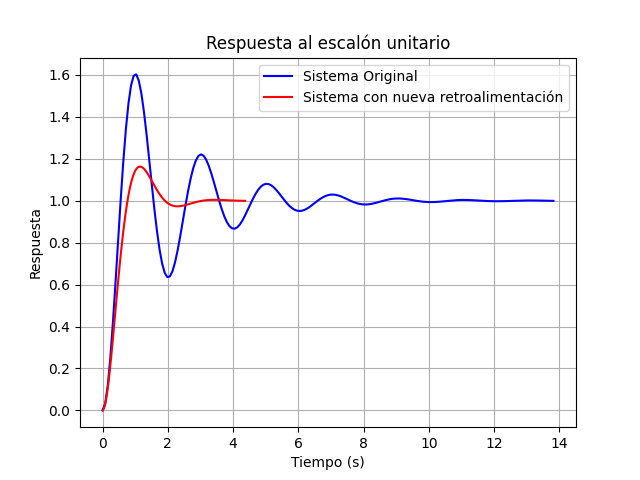
\includegraphics[width=0.7\textwidth]{./figures/Figura 6 ejercicio 5.png}
	\caption{Respuesta al escalón unitario de ambos sistemas}
\end{figure}

\newpage

\section{Problema 6: Considerando el sistema de la Figura 7, determine el valor de k , de modo que el factor de
  amortiguamiento sea 0,5. Basado en esto, obtenga el tiempo de levantamiento tr , el tiempo
  peak tp , el sobrepaso máximo Mp , y el tiempo de asentamiento ts , en la respuesta al escalón
  unitario. Obtenga analíticamente y muestre la respuesta en el tiempo (computacionalmente).}

\begin{figure}[h]
	\centering
	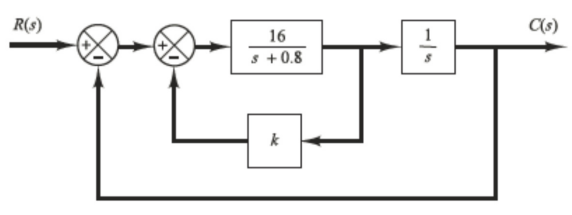
\includegraphics[width=0.8\textwidth]{./figures/Figura 7 ejercicio 6.png}
	\caption{Sistema de la Figura 7}
\end{figure}


La función de transferencia del sistema en la Figura 7 es:

\[
	G(s) = \frac{16}{s^2 + (0.8 + 16k)s + 16}
\]

\subsection{Determinación del valor de \texorpdfstring{\(k\)}{k}}

Para un sistema de segundo orden, la ecuación característica estándar es:

\[
	s^2 + 2\zeta \omega_n s + \omega_n^2 = 0
\]

Donde:
\begin{itemize}
	\item \(\zeta = 0.5\) (factor de amortiguamiento relativo),
	\item \(\omega_n\) es la frecuencia natural no amortiguada.
\end{itemize}

La ecuación característica del sistema será:

\[
	s^2 + (0.8 + 16k)s + 16 = 0
\]

El factor de amortiguamiento está relacionado con la frecuencia natural y la constante del término lineal en \(s\) por la fórmula:

\[
	2\zeta \omega_n = 0.8 + 16k
\]

Sustituyendo \(\zeta = 0.5\) y \(\omega_n = 4\):

\[
	2(0.5)(4) = 0.8 + 16k \quad \Rightarrow \quad 4 = 0.8 + 16k
\]
\[
	16k = 3.2 \quad \Rightarrow \quad k = \frac{3.2}{16} = 0.2
\]

\subsection{Cálculo de parámetros de la respuesta al escalón unitario}

\subsubsection{Tiempo de levantamiento \texorpdfstring{\(t_r\)}{tr}}

Frecuencia natural amortiguada \(\omega_d\):

\[
	\omega_d = \omega_n \sqrt{1 - \zeta^2} = 4 \sqrt{1 - (0.5)^2} = 4 \sqrt{0.75} = 4 \times 0.866 = 3.464
\]

El tiempo de levantamiento es el tiempo que tarda la salida en pasar del 10\% al 90\% del valor final. Para un sistema subamortiguado con \(\zeta = 0.5\), una aproximación es:

\[
	t_r \approx \frac{\pi - \arccos(\zeta)}{\omega_d} = \frac{\pi - \frac{\pi}{3}}{3.464} \approx 0.604 \, \text{segundos}
\]

\subsubsection{Tiempo peak \texorpdfstring{\(t_p\)}{tp}}

El tiempo peak es el tiempo que tarda la respuesta en alcanzar su primer máximo. Para un sistema de segundo orden:

\[
	t_p = \frac{\pi}{\omega_d} = \frac{\pi}{3.464} \approx 0.907 \, \text{segundos}
\]

\subsubsection{Sobrepaso máximo \texorpdfstring{\(M_p\)}{Mp}}

El sobrepaso máximo se puede calcular con la siguiente fórmula para un sistema de segundo orden:

\[
	M_p = e^{\left(\frac{-\pi \zeta}{\sqrt{1 - \zeta^2}}\right)} = e^{\left(\frac{-\pi (0.5)}{\sqrt{1 - (0.5)^2}}\right)} = e^{\left(\frac{-1.57}{0.866}\right)} \approx 16.3\%
\]

\subsubsection{Tiempo de asentamiento \texorpdfstring{\(t_s\)}{ts}}

El tiempo de asentamiento es el tiempo que tarda la respuesta en quedarse dentro de un 2\% del valor final. Para un sistema de segundo orden, el tiempo de asentamiento se aproxima como:

\[
	t_s \approx \frac{4}{\zeta \omega_n} = \frac{4}{0.5 \times 4} = 2 \, \text{segundos}
\]

\subsection{Simulación computacional}

Implementación computacional en Python
\begin{lstlisting}[language=Python]
import control as ctrl
import matplotlib.pyplot as plt

# Parametros del sistema
k = 0.2  # Valor de k determinado
num = [16]
den = [1, 0.8 + 16*k, 16]

# Crear el sistema en lazo cerrado
sys = ctrl.TransferFunction(num, den)

# Simulacion de la respuesta al escalon
t, y = ctrl.step_response(sys)

# Graficar la respuesta
plt.plot(t, y, label='Respuesta al escalon unitario')
plt.title('Respuesta al escalon unitario (k = 0.2)')
plt.xlabel('Tiempo (s)')
plt.ylabel('Respuesta')
plt.axvline(x=0.604, color='red', linestyle='--', label='Tiempo de levantamiento (Tr) 0.604 [s]')
plt.axvline(x=0.907, color='green', linestyle='--', label='Tiempo peak (Tp) 0.907 [s]')
plt.axvline(x=2, color='purple', linestyle='--', label='Tiempo de asentamiento (Ts) 2 [s]')
plt.plot([], [], ' ', label='Sobrepaso 16.3%')
plt.grid()
plt.legend() 
plt.show()
\end{lstlisting}

\begin{figure}[h]
	\centering
	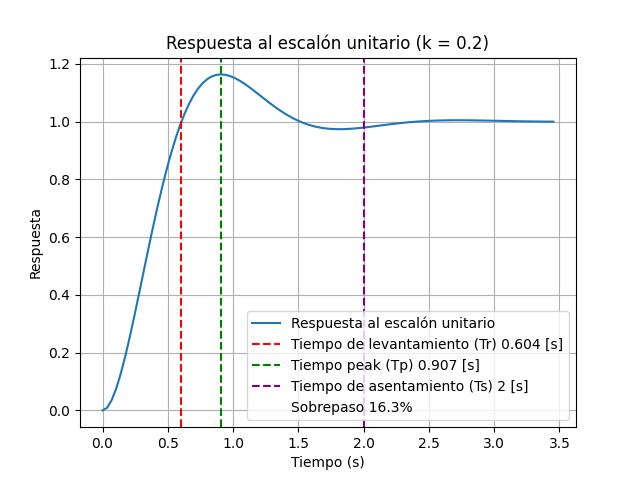
\includegraphics[width=0.7\textwidth]{./figures/Figura 8 ejercicio 6.png}
	\caption{Respuesta al escalón unitario del sistema con \(k = 0.2\)}
\end{figure}


Este código genera la respuesta al escalón unitario y te permite analizar visualmente cómo se comporta el sistema con el valor \(k = 0.2\).

\section{Problema 7: Las Figuras 9 muestran tres sistemas. El sistema I es un sistema de control de posición; el
  sistema II es un sistema de control de posición con un control PD; y el sistema III es un sistema
  de control de posición con retroalimentación de velocidad.
  Compare las respuestas a un escalón unitario e impulso unitario de los tres sistemas (computacionalmente, y ojalá en una misma gráfica). ¿Qué sistema es mejor con respecto a la velocidad
  de respuesta, y sobre el sobrepaso (elongación) máxima, en la respuesta al escalón? }


\begin{figure}[h]
	\centering
	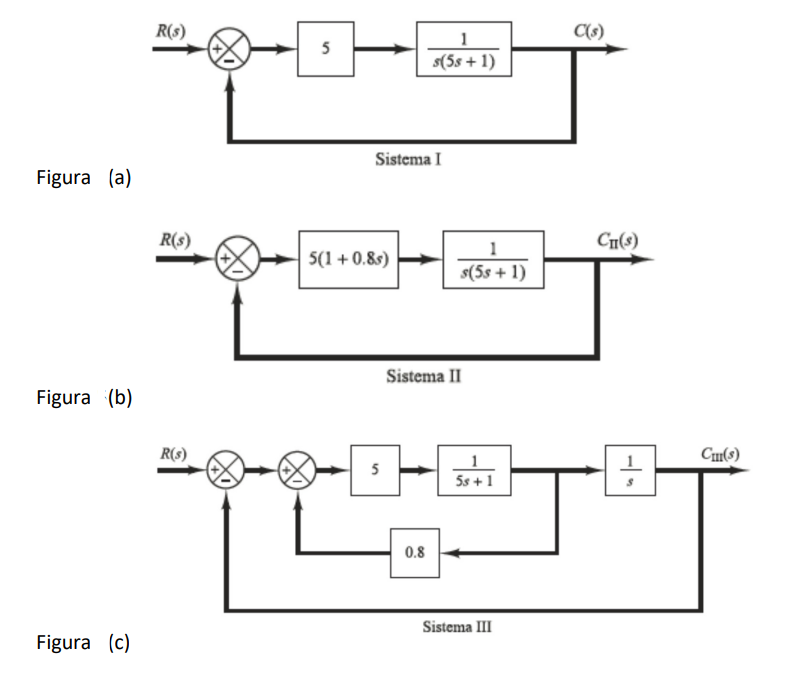
\includegraphics[width=0.8\textwidth]{./figures/Figura 9 ejercicio 7.png}
	\caption{Sistemas I, II y III}
\end{figure}

\newpage

\subsection{Funciones de transferencia de los sistemas}

\begin{equation}
	\text{a) } \frac{5}{s(5s+1)} = \frac{\frac{5}{s(5s+1)}}{1 + \frac{s}{s(5s+1)}} = \frac{5}{s(5s+1) + s}
\end{equation}

\begin{equation}
	\text{b) } \frac{5(1+0.8s)}{s(5s+1)} = \frac{\frac{5(1+0.8s)}{s(5s+1)}}{1 + \frac{5(1+0.8s)}{s(5s+1)}} = \frac{5(1+0.8s)}{s(5s+1) + 5(1+0.8s)}
\end{equation}

\begin{equation}
	\text{c) } \frac{5}{5s+1} = \frac{\frac{5}{5s+1}}{1 + \frac{4}{5s+1}} = \frac{1}{s+1} = \frac{\frac{1}{s+1}}{1 + \frac{1}{s^2+s}} = \frac{1}{s^2 + s + 1}
\end{equation}


Implementación computacional en Python
\begin{lstlisting}[language=Python]
	import numpy as np
	import matplotlib.pyplot as plt
	from scipy.signal import TransferFunction, step, impulse
	
	# Definir las funciones de transferencia usando scipy.signal.TransferFunction
	G_a = TransferFunction([5], [5, 1, 5])  # Sistema I: Control de posicion
	G_b = TransferFunction([4, 5], [5, 5, 5])  # Sistema II: Control de posicion con control PD
	G_c = TransferFunction([1], [1, 1, 1])  # Sistema III: Control de posicion con retroalimentacion de velocidad
	
	# Determinar el tiempo maximo de simulacion basado en las respuestas al escalon
	_, step_response_a = step(G_a)
	_, step_response_b = step(G_b)
	_, step_response_c = step(G_c)
	
	# Determinar el tiempo maximo de simulacion
	t_max = max(len(step_response_a), len(step_response_b), len(step_response_c))
	
	# Crear un vector de tiempo adecuado
	t = np.linspace(0, t_max, 1000)
	
	# Simulacion de la respuesta a un escalon unitario
	t_out_a, step_response_a = step(G_a, T=t)
	t_out_b, step_response_b = step(G_b, T=t)
	t_out_c, step_response_c = step(G_c, T=t)
	
	# Simulacion de la respuesta a un impulso unitario
	t_out_a_imp, impulse_response_a = impulse(G_a, T=t)
	t_out_b_imp, impulse_response_b = impulse(G_b, T=t)
	t_out_c_imp, impulse_response_c = impulse(G_c, T=t)
	
	# Graficar las respuestas al escalon
	plt.figure(figsize=(12, 8))
	
	plt.subplot(2, 1, 1)
	plt.plot(t_out_a, step_response_a, label='Sistema I - Escalon')
	plt.plot(t_out_b, step_response_b, label='Sistema II - Escalon')
	plt.plot(t_out_c, step_response_c, label='Sistema III - Escalon')
	plt.title('Respuesta al Escalon Unitario')
	plt.xlabel('Tiempo (s)')
	plt.ylabel('Amplitud')
	plt.legend()
	plt.grid()
	
	# Graficar las respuestas al impulso
	plt.subplot(2, 1, 2)
	plt.plot(t_out_a_imp, impulse_response_a, label='Sistema I - Impulso')
	plt.plot(t_out_b_imp, impulse_response_b, label='Sistema II - Impulso')
	plt.plot(t_out_c_imp, impulse_response_c, label='Sistema III - Impulso')
	plt.title('Respuesta al Impulso Unitario')
	plt.xlabel('Tiempo (s)')
	plt.ylabel('Amplitud')
	plt.legend()
	plt.grid()
	
	plt.tight_layout()
	plt.show()
\end{lstlisting}

\begin{figure}[h]
	\centering
	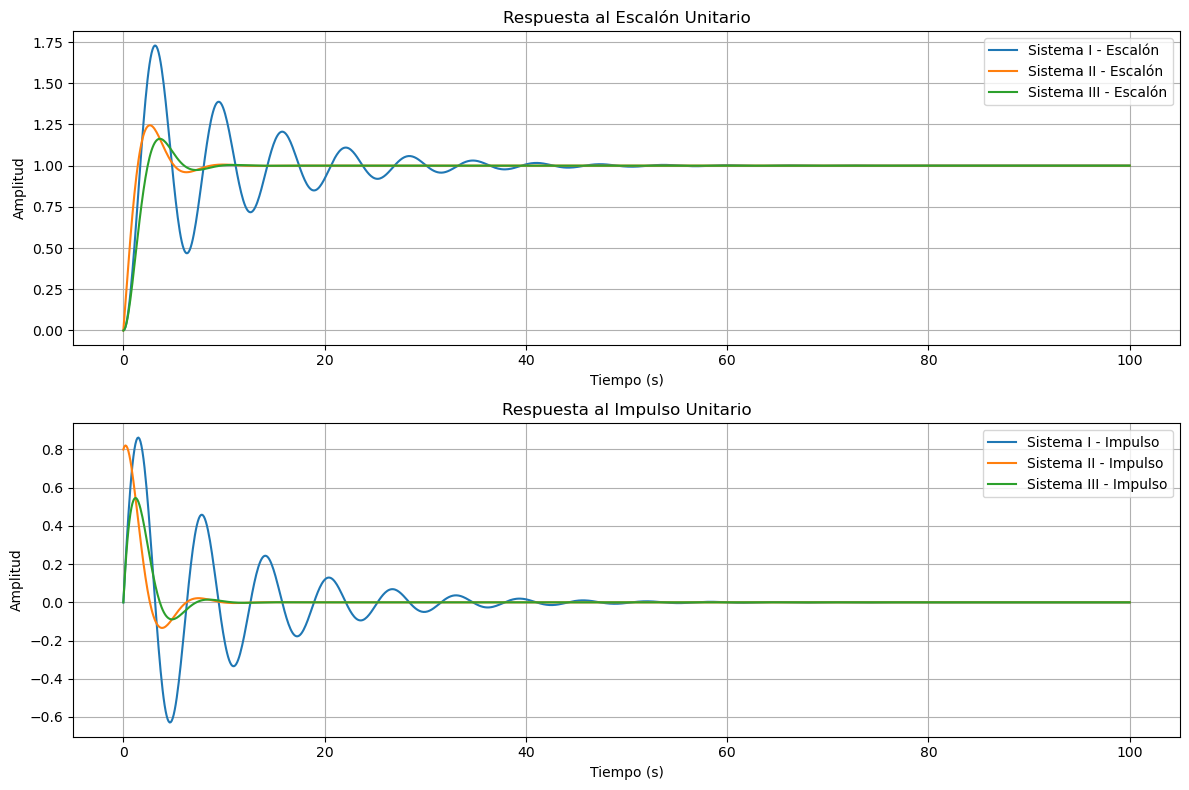
\includegraphics[width=1\textwidth]{./figures/Figura 10 ejercicio 7.png}
	\caption{Respuestas al escalón unitario de los sistemas I, II y III}
\end{figure}

\newpage

\subsection{Análisis de las respuestas al escalón e impulso unitario}

A partir de los gráficos de las respuestas al \textbf{escalón unitario} y al \textbf{impulso unitario} de los tres sistemas, se puede realizar el siguiente análisis:

\subsection{Respuesta al escalón unitario}



\begin{itemize}
	\item \textbf{Sistema I (azul)}:
	      \begin{itemize}
		      \item Tiene el \textbf{mayor sobrepaso} y un comportamiento oscilatorio prolongado, lo que indica una baja amortiguación y una respuesta menos controlada.
		      \item Su \textbf{velocidad de respuesta} es menor que la de los otros dos sistemas, ya que tarda más en estabilizarse.
	      \end{itemize}
	\item \textbf{Sistema II (naranja)}:
	      \begin{itemize}
		      \item Presenta un \textbf{sobrepaso menor} que el Sistema I y una mejor estabilidad.
		      \item Su \textbf{velocidad de respuesta} es más rápida que la del Sistema I, estabilizándose con menos oscilaciones.
	      \end{itemize}
	\item \textbf{Sistema III (verde)}:
	      \begin{itemize}
		      \item Este sistema tiene \textbf{prácticamente nulo sobrepaso} y se estabiliza rápidamente sin oscilaciones significativas.
		      \item Es el \textbf{más estable} de los tres sistemas, pero su \textbf{velocidad de respuesta} es ligeramente más lenta que la del Sistema II debido a su fuerte amortiguación.
	      \end{itemize}
\end{itemize}

\subsection{Respuesta al impulso unitario}

Los patrones observados son similares a los de la respuesta al escalón. El \textbf{Sistema I} tiene el mayor sobrepaso y la mayor oscilación, mientras que el \textbf{Sistema III} es el más estable, con una rápida estabilización.

\subsection{Conclusión}

\begin{itemize}
	\item \textbf{Velocidad de respuesta}: El \textbf{Sistema II} parece tener la mejor velocidad de respuesta, ya que alcanza su estado estable más rápidamente que los demás con un control razonable del sobrepaso.
	\item \textbf{Sobrepaso máximo}: El \textbf{Sistema III} es el que tiene el menor sobrepaso y es el más estable en ambas respuestas (escalón e impulso).
\end{itemize}

Por lo tanto, si se busca una respuesta más rápida, el \textbf{Sistema II} es el más adecuado. Sin embargo, si la prioridad es minimizar el sobrepaso y maximizar la estabilidad, el \textbf{Sistema III} es el más recomendable.

\end{document}